We present our framework to ensure that all momentous events in the vehicle lifecycle are efficiently and securely stored and retrieved to
ensure that network trust and integrity are maintained. The framework uses the Vehicle Identification Number (VIN), a unique identifier
assigned to the vehicle in production. In this section, the methods and design decisions behind the framework will be discussed.

\subsection{Stakeholders}
\begin{figure}[H]
	\centering
	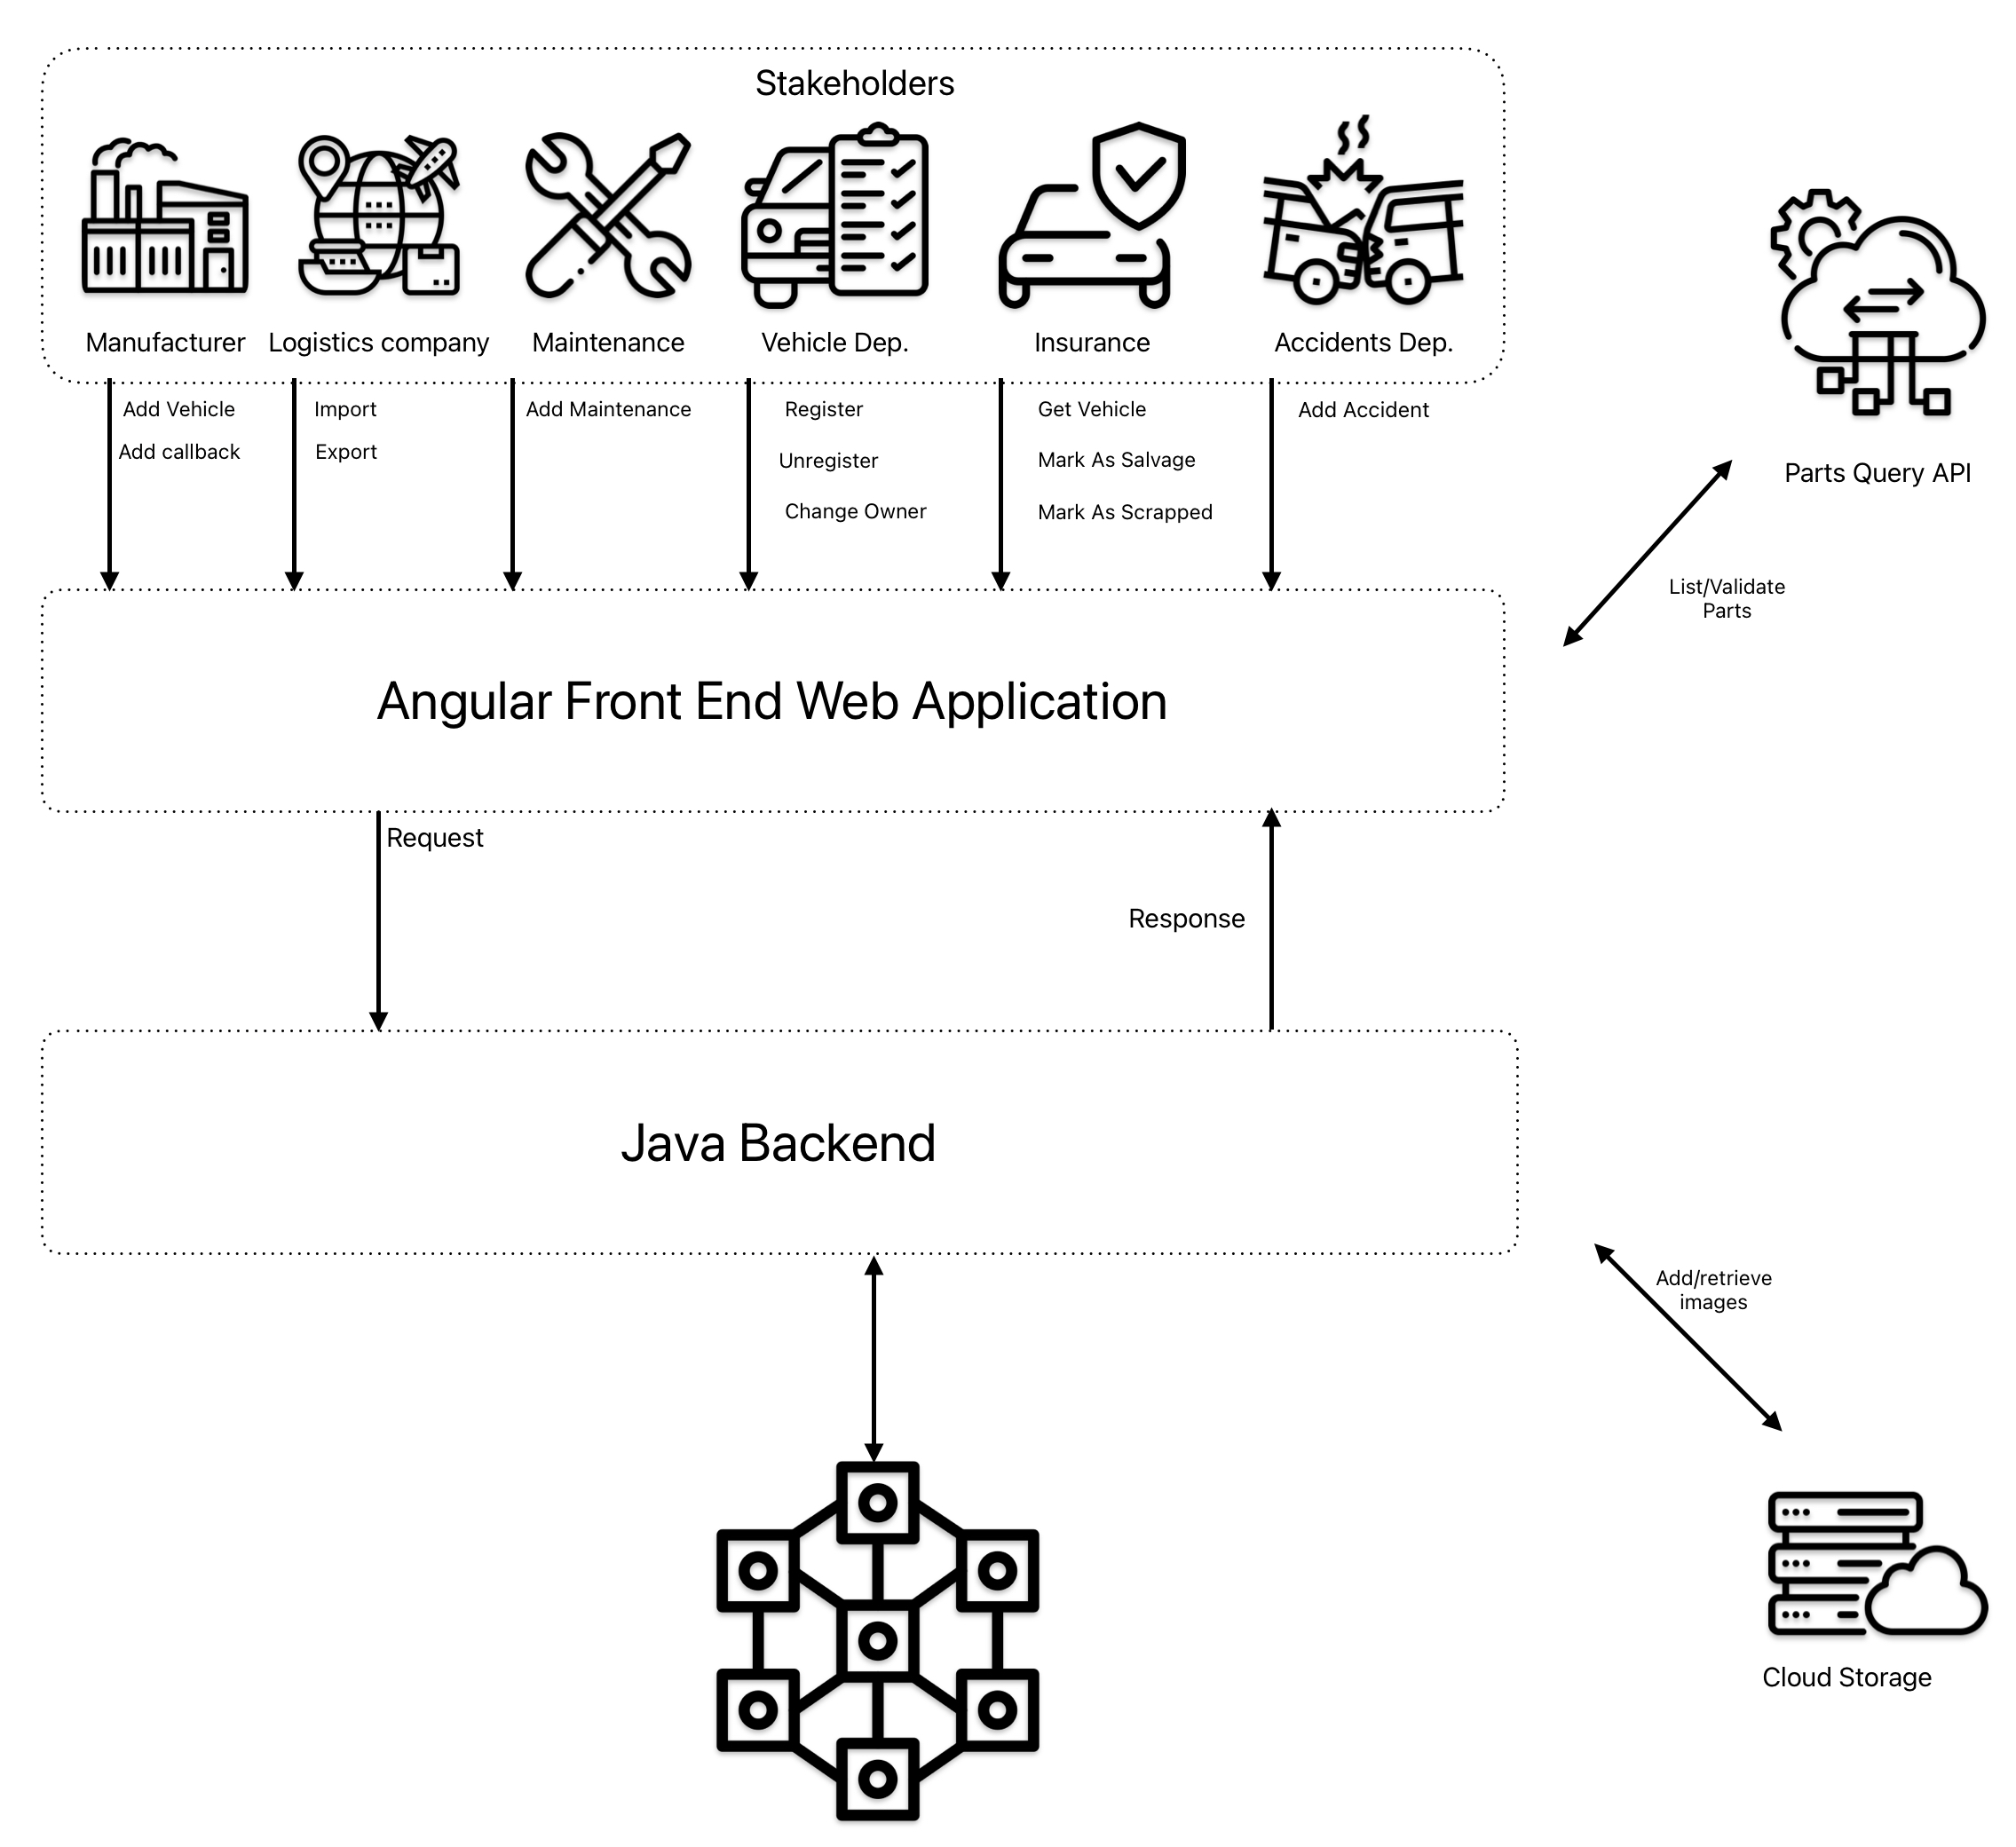
\includegraphics[width=\linewidth]{figures/sys-framework}
	\caption{System Framework.}
	\label{fig:sys-framework}
\end{figure}
The framework has six main stakeholders with specific operations for each. As figure \ref{fig:df-sys-framework} shows, the stakeholders are:
\begin{enumerate}
	\item Manufacturer, which can add new vehicles to the network and add vehicle callbacks.
	\item Logistics company, which has import and export operations.
	\item Maintenance shop, and it can only add new maintenance records.
	\item Vehicle department has three operations; register vehicles, unregister vehicles, change vehicle ownership.
	\item Insurance company, it can mark a vehicle as scrapped or salvaged and retrieve vehicle information.
	\item Accidents department has an operation to add vehicle accident records.
\end{enumerate}
\begin{figure}[H]
	\centering
	\begin{tikzpicture}[scale=0.5,transform shape]
		\tikzstyle{actor} = [draw, thick, minimum width=1cm, minimum height=1cm]
		\tikzstyle{message} = [draw, thick, -latex]
		\tikzstyle{instance} = [draw, thick, dashed, minimum height=6cm]

		\node[actor] (StakeHolder) {StakeHolders};
		\node[actor, below=1.5cm of StakeHolder] (Manufacturer) {Manufacturer};
		\node[actor, below=1.4 of Manufacturer] (Maintenance) {Maintenance Shop};
		\node[actor, below=1.4 of Maintenance] (Accidents) {Accidents Department};
		\node[actor, below=1.4 of Accidents] (Vehicles) {Vehicles Department};
		\node[actor, below=1.4 of Vehicles] (Insurance) {Insurance Companies};
		\node[actor, below=1.2 of Insurance] (Logistics) {Logistics Companies};
		\node[actor, right=1cm of StakeHolder] (Webpage) {Angular Webpage};
		\node[actor, right=1cm of Webpage] (BackEnd) {Back-End};
		\node[actor, right=1.5cm of BackEnd] (HyperLedger) {HyperLedger};
		\node[actor, right=1cm of HyperLedger] (Ledger) {Ledger};
		\node[actor, right=1cm of Ledger] (RestServices) {Rest Services};
		\node[actor, right=1cm of RestServices] (CloudStorage) {Cloud Storage};

		\draw[instance] (StakeHolder) -- ++(0,-2);
		\draw[instance] (Manufacturer) -- ++(0,-2);
		\draw[instance] (Maintenance) -- ++(0,-2);
		\draw[instance] (Accidents) -- ++(0,-2);
		\draw[instance] (Vehicles) -- ++(0,-2);
		\draw[instance] (Insurance) -- ++(0,-1.65);
		\draw[instance] (Webpage) -- ++(0,-15);
		\draw[instance] (BackEnd) -- ++(0,-15);
		\draw[instance] (HyperLedger) -- ++(0,-15);
		\draw[instance] (Ledger) -- ++(0,-15);
		\draw[instance] (RestServices) -- ++(0,-15);
		\draw[instance] (CloudStorage) -- ++(0,-15);

		\draw[message] ($(StakeHolder)-(0,1.3)$) -- ($(Webpage)-(0,1.3)$) node[midway, above] {Uses};
		\draw[message] ($(Webpage)-(0,8)$) -- ($(BackEnd)-(0,8)$) node[midway, above] {Request};
		\draw[message] ($(BackEnd)-(0,13)$) -- ($(Webpage)-(0,13)$) node[midway, above] {Response};
		\draw[message] ($(BackEnd)-(0,9)$) -- ($(HyperLedger)-(0,9)$) node[midway, above] {Submit Transaction};
		\draw[message] ($(HyperLedger)-(0,12)$) -- ($(BackEnd)-(0,12)$) node[midway, above] {Query Transaction};
		\draw[message] ($(Webpage)-(0,3.5)$) -- ($(RestServices)-(0,3.5)$) node[midway, above] {Request};
		\draw[message] ($(RestServices)-(0,5)$) -- ($(Webpage)-(0,5)$) node[midway, above] {Response};
		\draw[message] ($(HyperLedger)-(0,10)$) -- ($(Ledger)-(0,10)$) node[midway, above] {Add Block};
		\draw[message] ($(Ledger)-(0,11)$) -- ($(HyperLedger)-(0,11)$) node[midway, above] {Retrieve Data};
		\draw[message] ($(BackEnd)-(0,6)$) -- ($(CloudStorage)-(0,6)$) node[midway, above] {Upload Image};
		\draw[message] ($(CloudStorage)-(0,7)$) -- ($(BackEnd)-(0,7)$) node[midway, above] {Download Image};

	\end{tikzpicture}
	\caption{Framework Dataflow.}
	\label{fig:df-sys-framework}
\end{figure}

\begin{table}[H]
	\caption{Chaincode validations.}
	\label{tab:chaincode-validations}
	\tiny
	\begin{tabularx}{\linewidth}{X|X|X}
		\toprule
		Stakeholder        & Chaincode        & Validations
		\\
		\toprule
		Manufacturer         & Create Vehicle   &  VIN is unique. \newline
		All initial data exist (Color, Country of origin, Production year, Model). \\
		\cmidrule{2-3}
		& Create Callback  & -                                                                                                       \\
		\midrule
		Logistic             & Import           & Vehicle is exported. \newline Vehicle exists in the same country. \newline Valid 
		Odometer.
		\\
		\cmidrule{2-3}
		& Export           & Vehicle not registered to an owner. \newline Valid Odometer.                                            \\
		\midrule
		Accidents Department & -                & -
		\\
		\midrule
		Vehicles Department  & Register         & Not registered to an owner. \newline Vehicle is imported. \newline Valid Odometer.
		\\
		\cmidrule{2-3}
		& Unregister       & Registered to an owner. \newline Valid Odometer.                                                        \\
		\cmidrule{2-3}
		& Change Ownership & Registered to an owner. \newline Seller is the owner. \newline Valid Odometer.                          \\
		\midrule
		Maintenance          & Add Maintenance  & Valid Odometer. \newline Genuine Part: \newline Have serial number. \newline
		Authenticity verified.     \\
		\midrule
		Insurance companies  & -                & -
		\\
		\bottomrule
	\end{tabularx}
\end{table}
As table \ref{tab:chaincode-validations}
shows, the framework has a set of validations for each type of stakeholders to ensure the validity of the transactions before
adding them to the ledger. These validations are the cornerstone of the framework, so every endorsing peer will have its chaincode deployed
on separate container or server to ensure it is security and integrity. Finally, endorsement is based on the majority consensus method and
the transaction is considered valid only if the initiation peer received approvals from at least 50\% of the network.
\begin{figure}[H]
	\centering
	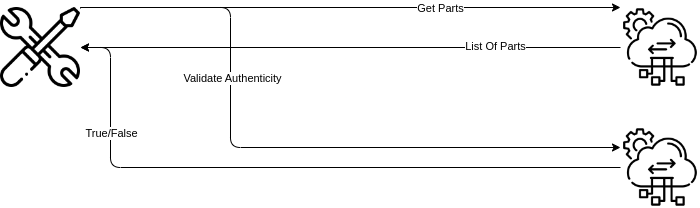
\includegraphics[width=\linewidth]{figures/parts-service-wf}
	\caption{Parts Query Service WorkFlow.}
	\label{fig:parts-query-wf}
\end{figure}

As figure \ref{fig:parts-query-wf}
shows, the framework uses a restful API to communicate with Parts Query API which is a Restful service deployed by vehicle
manufacturers with two endpoints to enable the framework to retrieve vehicles list of replacement parts and validate parts serial number in
case the manufacturer stated that it has a serial number. 


The framework is built on HL fabric framework as a hybrid BC where only users who the sufficient permissions can
add transactions based on their given role. To ensure transparency, vehicles reports are publicly available, and any individual
can query the data of any vehicle using its VIN without the need for credentials. 

\begin{figure}[H]
\centering
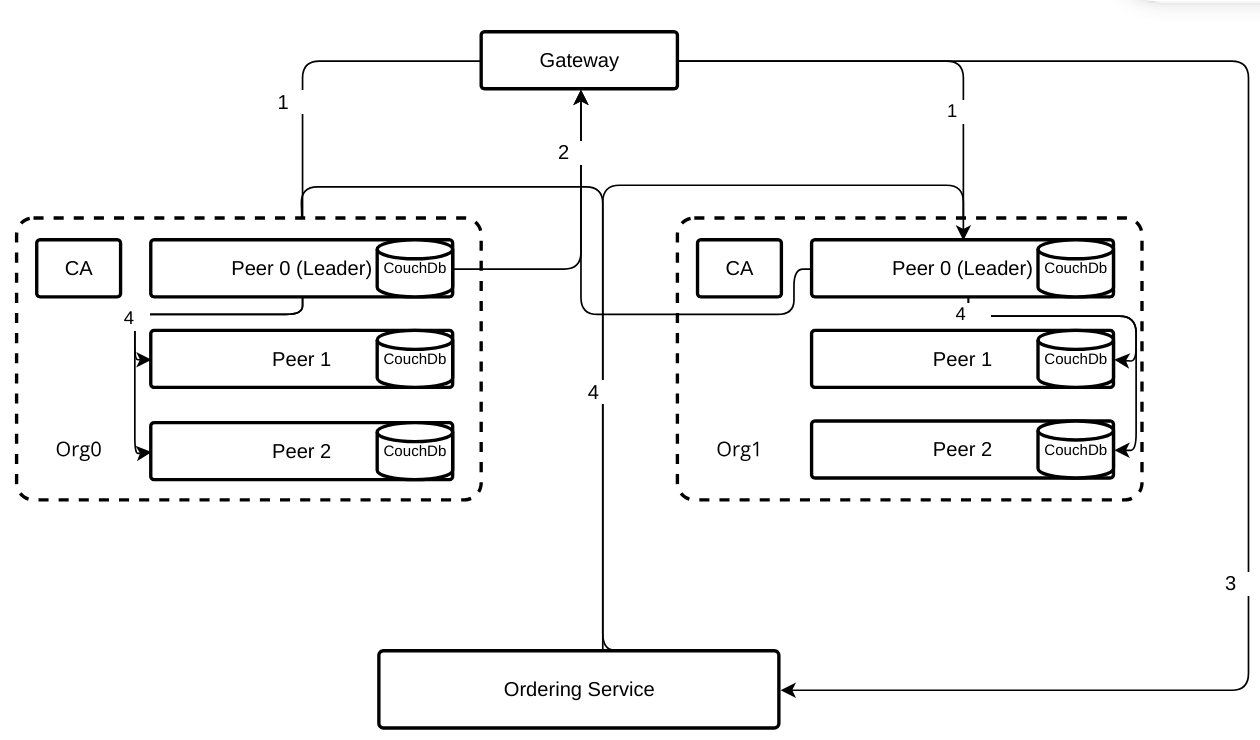
\includegraphics[width=\linewidth]{figures/hyper-ledger-flow}
\caption{Hyper Ledger Transaction Flow.}
\label{fig:hyper-ledger-wf}
\end{figure}
As figure~\ref{fig:hyper-ledger-wf}
show, the transaction moves in multiple stages before it is committed and we will dive into the flow as:
\begin{enumerate}
\item When the gateway receives the transaction request, it sends transaction proposal to the endorsing peers.
\item the endorsing peers simulate and validate the transaction, then it sends proposal response to the gateway.
\item when the gateway receives enough number of approvals it sends the transaction to the ordering service.
\item the ordering service maintains the transactions in a chronological order and when new block conditions are satisfied it sends
the new block to all peers to be committed.
\item the new block is now committed into the ledger.
\end{enumerate}
To enhance the performance of the peers and decrease the size of the transactions, an external
CouchDb is used to store the vehicle images. The images are encrypted using a unique cryptographic key generated for each
image, then its encrypted using base64 before uploading it to the external DB. The ledger will only contain the
image id the CouchDb and the decryption key, these measures ensures that images cannot be altered or modified if
a malicious party got access to the external DB. Moreover, the framework uses several security methods namely: spring security
with Json Web Token to control user's authentication and authorization, nginx server to manage the load balancing between server
nodes and prevent attacks such as Denial of Service (DoS), and the use of Transport Layer Security
(TLS) to secure all communications within the framework. Finally, the implementation of these methods ensures the framework security and
integrity. 